\section{Failure Analysis and Yield Improvement}

\subsection{Initial Observation}
The first production lots showed $\sim$65\% yield. Wafer test was dominated by \textbf{Pause Refresh Fail (Bin5)}. Defects appeared as uniformly scattered single-bit errors across the wafer (weak clustering, no edge/line signature). Storage-node capacitance met spec; SEM cross-sections at failed cells revealed no structural anomaly. Other CDs/films/electricals were within spec.

\begin{figure}[t]
  \centering
  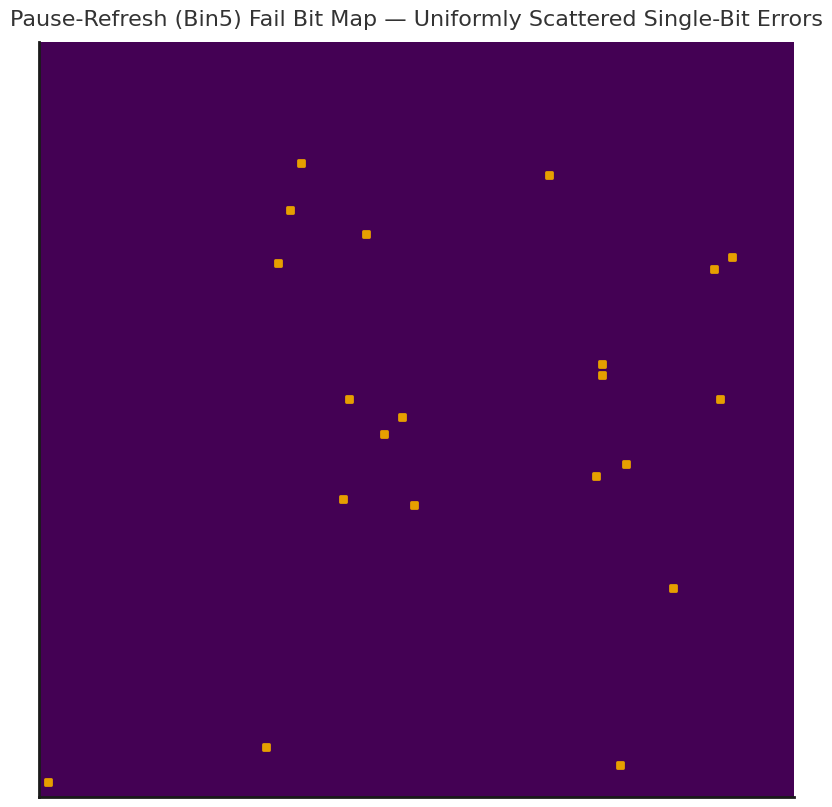
\includegraphics[width=\columnwidth]{fail_bitmap_bin5}
  \caption{Typical fail bit map under pause-refresh test (Bin5).
  Uniformly scattered single-bit errors are observed without edge/line signatures.}
  \label{fig:fail_bitmap}
\end{figure}

\subsection{Hypothesis (Failure Model)}
Directly measurable leakages were normal, suggesting a subtle leakage path. We hypothesized increased leakage at the \textbf{storage-node contact $n^+/p^-$ junction}. After gate etch, a remnant gate oxide on S/D active is repeatedly exposed to resist-stripping \emph{ashing} during multiple LDD steps. Cumulative plasma damage makes the oxide locally porous and can extend damage into the diffusion, creating minute leakage paths. This explains random single-bit distribution without visible structural defects.

% === Fig.2 (minimal TikZ) ===
\begin{figure}[t]
  \centering
  \begin{tikzpicture}[x=4cm,y=3cm,line cap=round,line join=round,>=Latex]
    % 表面
    \draw[black!50] (0,0) -- (1.10,0);

    % p- 基板
    \draw[fill=black!5,draw=black!40] (0,-0.35) rectangle (1.10,-0.75);
    \node[anchor=west,scale=0.7] at (0.02,-0.68) {$p^{-}$ substrate};

    % WL(ポリ)
    \draw[fill=black!20,draw=black] (0.12,0.06) rectangle (0.28,0.30);
    \node[scale=0.7] at (0.20,0.36) {WL};

    % n+ 拡散
    \draw[fill=cyan!15,draw=cyan!60!black] (0.35,-0.02) rectangle (0.70,-0.35);
    \node[scale=0.7] at (0.525,-0.28) {$n^{+}$};

    % LOCOS(簡易の盛り上がり)
    \draw[draw=orange!60!black,fill=orange!15]
      (0.70,0) .. controls (0.82,0.10) and (0.96,0.10) .. (1.08,0)
      -- (1.08,-0.20) -- (0.70,-0.20) -- cycle;
    \node[scale=0.7] at (0.98,0.12) {LOCOS};

    % SN(金属)と縦コンタクト
    \draw[fill=gray!30,draw=gray!70] (0.54,0.55) rectangle (0.74,0.70);
    \node[scale=0.7] at (0.64,0.76) {SN};
    \draw[fill=gray!30,draw=gray!70] (0.635,0.30) rectangle (0.655,0.55);
    % n+ 上への着地を示す短線
    \draw[gray!70,thick] (0.58,0.30) -- (0.70,0.30);
    \node[anchor=west,scale=0.7] at (0.72,0.30) {storage-node contact};

    % リーク経路(最小要素:1本の点線矢印)
    \draw[very thick,black!70,dashed,-{Latex[length=2mm]}]
      (0.70,0.30) .. controls (0.66,0.10) and (0.62,-0.10) .. (0.58,-0.48);
    \node[anchor=west,scale=0.7] at (0.72,0.18) {leakage path};
  \end{tikzpicture}

  \caption{Minimal sketch of storage-node contact ($n^+/p^-$) leakage:
  WL--$n^+$--LOCOS layout, SN contact landing on $n^+$, and a dashed leakage
  path into the $p^-$ substrate.}
  \label{fig:fig2_min}
\end{figure}

\subsection{Countermeasures}
\begin{itemize}
  \item \textbf{Process}: Replace resist stripping in LDD steps from plasma ashing to \textbf{wet stripping (sulfuric-based)} to eliminate plasma damage. 
  \item \textbf{Integration hygiene}: Confirm downstream photo cleanliness and avoid residue risks with the wet strip.
\end{itemize}

\subsection{Effectiveness}
Yield improved from $\sim$65\% to \textbf{$\sim$80\%}. Uniformly scattered single-bit fails decreased markedly. Burn-in and retention/reliability passed; the final recipe was fixed for volume production.

% === Yield-by-lot (step improvement at countermeasure) ===
\begin{figure}[t]
\centering
\pgfplotstableread[col sep=comma]{data/yield_lot.csv}\yieldtbl
\begin{tikzpicture}
\begin{axis}[
  width=\columnwidth, height=0.58\columnwidth,
  xlabel={Lot ID}, ylabel={Yield [\%]},
  ymin=50, ymax=95,
  xmin=0.5, xmax=12.5,
  grid=both,
  xtick=data,
  xticklabels from table={\yieldtbl}{lot},
  xticklabel style={rotate=45, anchor=east},
]
  % データ描画
  \addplot+[mark=*] table[x expr=\coordindex+1, y=yield]{\yieldtbl};

  % 対策境界: lot04とlot05の間
  \draw[dashed] (axis cs:4.5,50) -- (axis cs:4.5,95);
  \node[anchor=west, font=\footnotesize] at (axis cs:4.55,92)
    {Countermeasure};
\end{axis}
\end{tikzpicture}
\caption{Yield step improvement at the countermeasure boundary
between \texttt{lot04} and \texttt{lot05}. Yield jumps from $\sim$62--63\% 
(lot01--lot04) to $\sim$82--84\% (lot05 onward) after changing 
LDD resist stripping from ashing to wet stripping.}
\label{fig:yield}
\end{figure}
